\documentclass{article}
\usepackage{indentfirst}
\usepackage{hyperref}
\hypersetup{
	colorlinks=true,
	urlcolor=blue,
	pdftitle={How to Use the User Settings GUI},
}
\usepackage{graphicx}
\graphicspath{ {./images/} }

\begin{document}
\begin{center}
\Large{How to Use the User Settings GUI}
\end{center}

Upon opening the application you will see a simple port selection page, open the dropdown and select the controller (usually there won't be a lot of Serial Ports to choose from). If none are showing up, make sure your USB cord is securely connected and press the Refresh Ports button.

\begin{center}
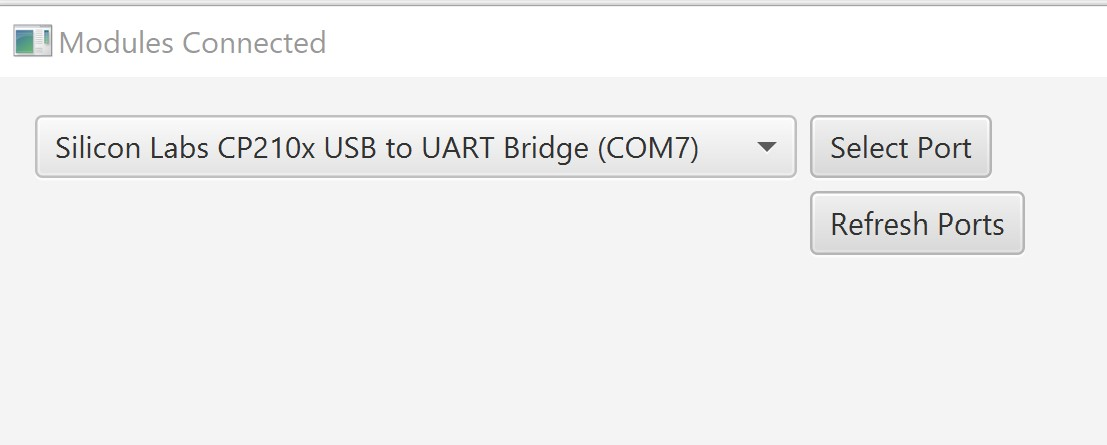
\includegraphics{SelectPort}
\end{center}

After selecting the proper port from the dropdown, hit the Select Port button. At this point the GUI will appear to freeze while it communicates with your controller, but should soon show the modules you have connected to your controller.

\begin{center}
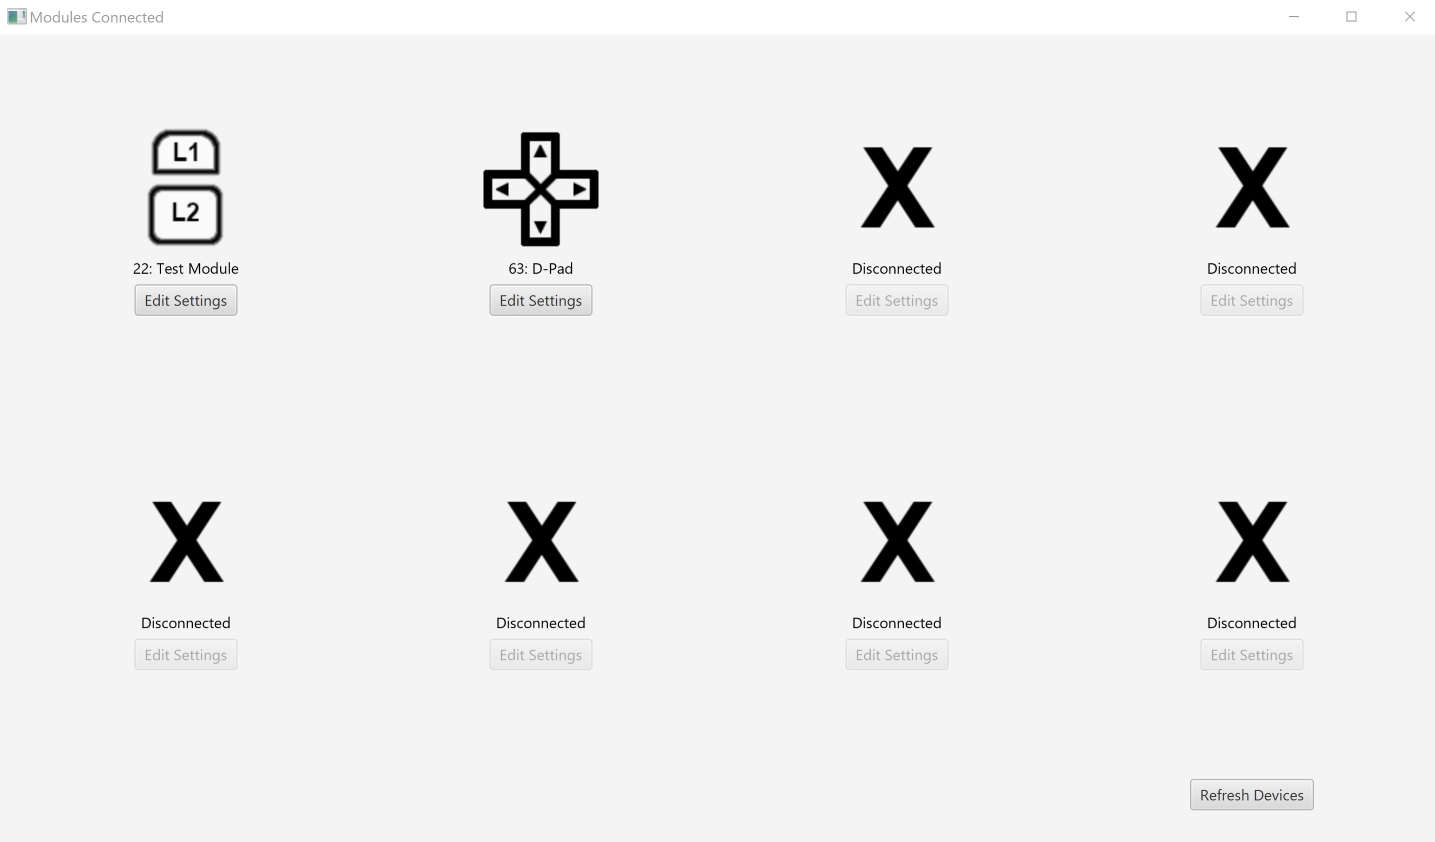
\includegraphics{ModulesPage}
\end{center}

Hit the Edit Settings button under the name of the module you would like to edit to open the module settings window.

\begin{center}
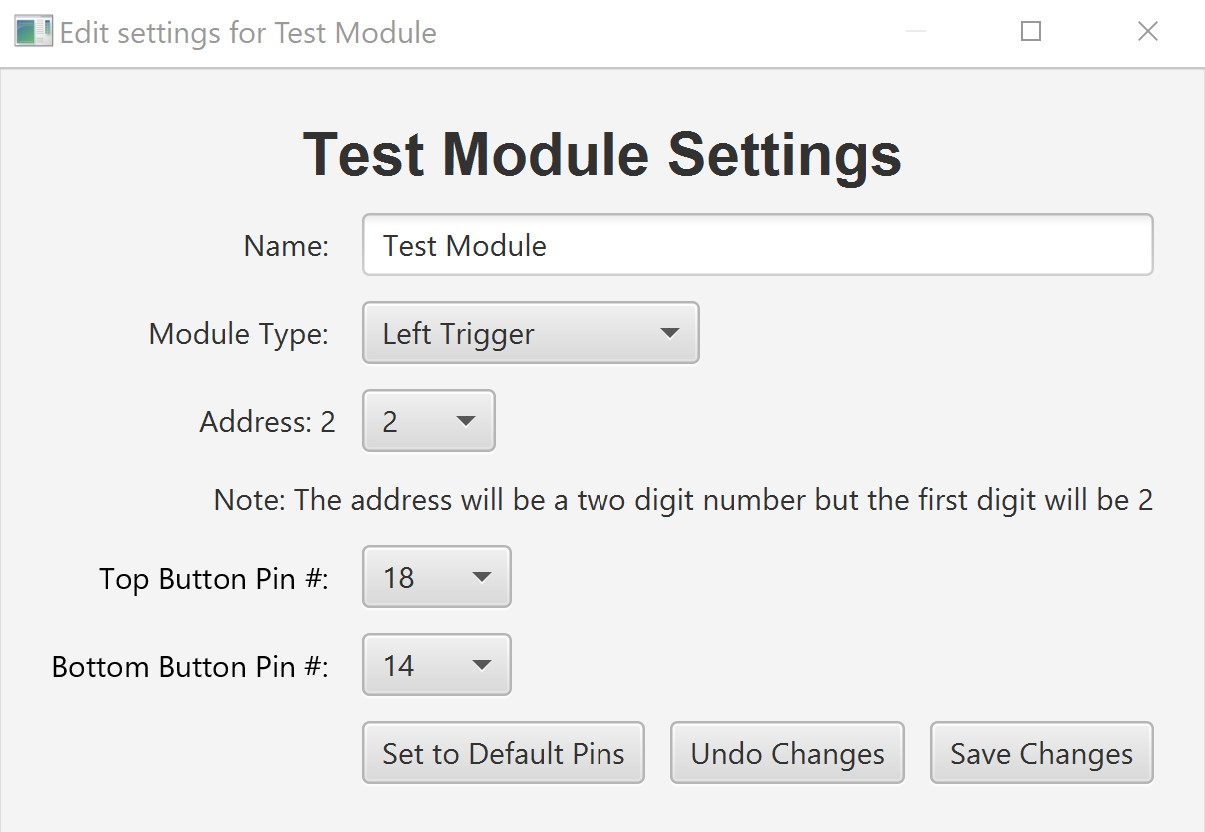
\includegraphics{ModuleSettings}
\end{center}

Here you can type in the name, select the module type, set an address, and configure the pins.

\begin{center}
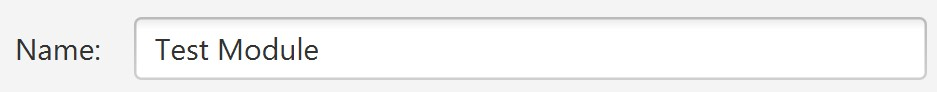
\includegraphics{NameField}
\end{center}
\textbf{Name} is only for your use, generally you will probably want to give it some sort of descriptive name. Names cannot contain semi-colons ( ; ), but can contain most other characters.

\begin{center}
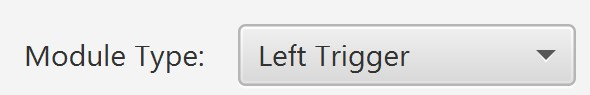
\includegraphics{ModTypeField}
\end{center}
\textbf{Module Type} will usually match the hardware you have, however you can select:
\begin{itemize}
  \item Whether a joystick should be considered the left or right joystick (since generally the left joystick is used for movement while the right is used to look around)
  \item Whether a trigger should be read as the left trigger or right trigger
  \item Whether a 4-button set up should be considered face buttons (A/B/X/Y or Square/Triangle/Circle/Cross) or a d-pad.
\end{itemize}
there is also an option for a custom module.

\begin{center}
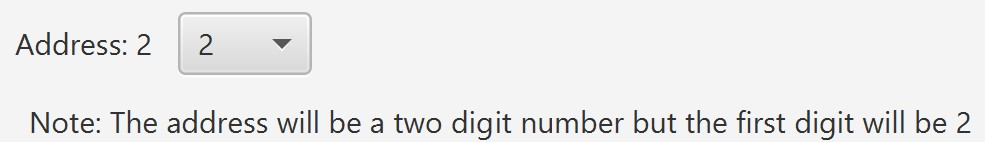
\includegraphics{AddrField}
\end{center}
\textbf{Address} mostly just needs to be unique, but we have certain ranges set for specific module types. Because of this, the tens-digit of our designed modules will be set by device type by the GUI (this is what the 'Note' below the address selection is referring to). If you are configuring a Feedback or Custom module you will have to set the address between 70 and 127, inclusive (meaning 70 and 127 are also valid addresses).

\begin{center}
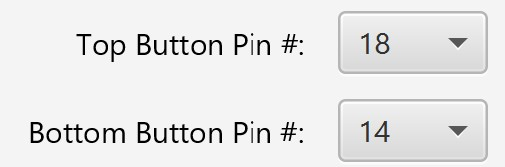
\includegraphics{PinsField1}
\end{center}
\textbf{Pins} will depend on the module type you are working with. In general, this will be important if you are using your own design for a module, or if you miswire a module and need to change the pin settings (ex. you accidentally wire the top button on a trigger to pin 17 instead of pin 18, instead of having to re-wire it you can just set the 'Top Button Pin \#' to 17).

\newpage
\begin{center}
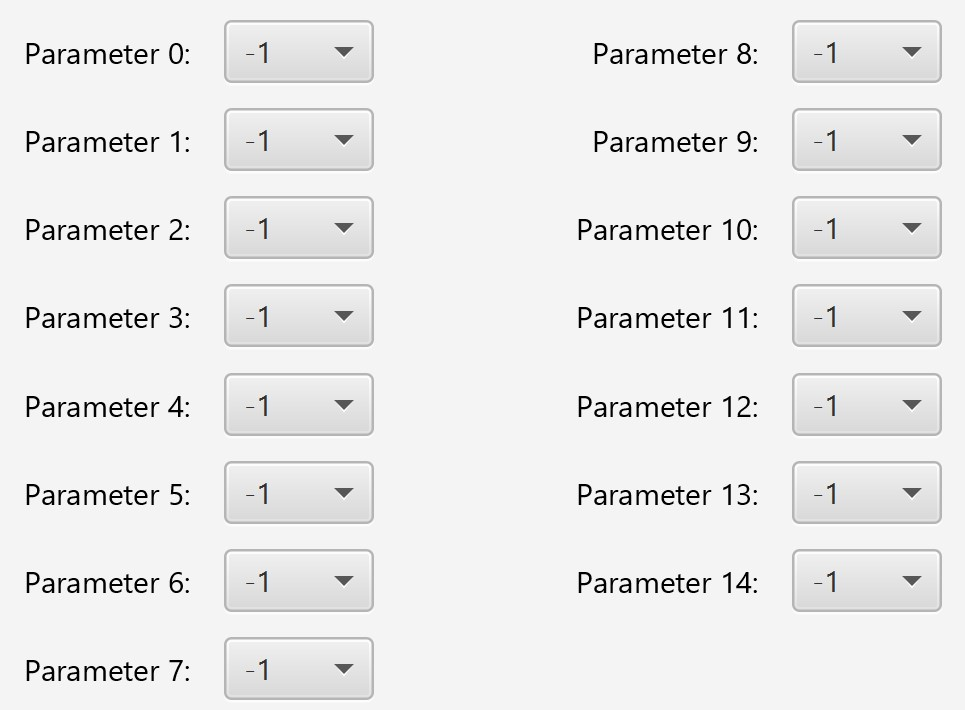
\includegraphics{PinsField2}
\end{center}
If you've selected 'Custom Module' or 'Feedback Device' you will get 15 pin settings dropdowns for you to configure based on your module's design. The details related to hardware design are beyond the scope of this guide.

\begin{center}
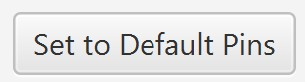
\includegraphics{DefaultBtn}
\end{center}
The 'Set to Default Pins' button will set all pin values to match our PCBs.

\begin{center}
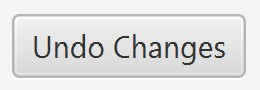
\includegraphics{UndoBtn}
\end{center}
The 'Undo Changes' button will reset all values to what the module currently has saved for its values.

\begin{center}
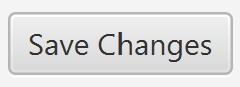
\includegraphics{SaveBtn}
\end{center}
When you are happy with the changes, you can hit the 'Save Changes' button. 
\begin{center}
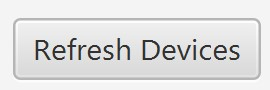
\includegraphics{RefreshBtn}
\end{center}
Please note, the GUI does not automatically refresh devices, so after saving you will have to hit the Refresh Devices buttons to see the changes that have been written to the module.

\end{document}